% -*- TeX -*- -*- UK -*- -*- Soft -*-

\chapter{Bayesian Glossary}
\label{chap:BayesianGlossary}


This material is taken from \cite{RavinKumarBayesianGlossary2019}, several refinements and corrections.

When reading Bayesian texts, or listening to lectures, terms like ''posterior'' or ''data'' are used, but often without explanation leaving the audience confused. I also find that even after learning the concepts once, its easy to mix them up. To that end I put together this glossary to serve as a quick reference to the terms, with examples. The writing is colloquial, for precise definitions I recommend the following references:
\begin{enumerate}
\item Bayesian Analysis with Python \cite{martin2018}. 
\item Bayesian Data Analysis \cite{gelmanbda04}.
\item Statistical Rethinking \cite{McElreath2015}. For further background I highly suggest purchasing his book and watching his lectures on YouTube.
\end{enumerate}

\section{Motivating Example: Proportion of water on a globe}

We will be using this example from Richard McElreath \cite{McElreath2015} to help define all terms. In his example, we want to know the proportion of water on a given globe. We make estimations by independent tosses of a globe, catching it, and seeing whether our right index finger is on water (W, probability $p$) or Land (L, probability $1-p$).  For this example assume the results to be \lstinline{W L W W W L W L W}.

We will be calculating some values, with the code shown in line with the text.
\begin{lstlisting}
    import numpy as np
    from scipy import stats
    import arviz as az
    import pymc3 as pm
    import matplotlib.pyplot as plt
    import seaborn as sns
    import pandas as pd
\end{lstlisting}

\section{Glossary}

\newthought{Data} in Bayesian analysis is the fixed truth of what has been observed. There is no uncertainty or probability. In our example the globe was tossed, the sequence of events observed is \lstinline{Water, Land, Water Water Water, Land, Water, Land, Water}.

\newthought{A Model} is a representation of some other thing.  In Bayesian analysis a model is a representation of the data generating process made of out mathematical distributions. Below is a model of the globe tossing example, written in pseudo mathematical notation.

\begin{lstlisting}
proportion_of_water=p=Uniform(0,1)
count_water_obs=Binomial(p,number_of_tosses)
\end{lstlisting}
It is important to know that models, unlike data, are not fixed and are completely human made. Two models can exist at the same time. For example, here is another model of the globe tosses:
\begin{lstlisting}
lamda=Uniform(0,1)
count_water_obs=Poisson(lamda)
\end{lstlisting}
Neither model is correct, nor is either model wrong! Both models are only a representation of the globe tossing, and justifying model choice is a core activity of Bayesian analysis.

\newthought{Bayes Theorem} is the probability event, taking into account past events that provide information about the event. The most generic formulation is 

\begin{equation}
P(A|B) = \frac{P(B|A)P(A)}{P(B)}
\end{equation}
A representation that I find more intuitive however is this one 

\begin{equation}
    P(\textrm{parameters}|\textrm{data}) = 
    \frac{P(\textrm{data}|\textrm{parameters})P(\textrm{parameters})} {P(\textrm{data})}
\end{equation}

Sometimes Bayes Theorem is written as shown below \cite{WikiPediaLikelihoodfunction2019}. This perhaps is the most ''technically correct'' because it differentiates between likelihood and probability. (See likelihood and probability glossary terms below)
\begin{equation}
    P(\textrm{parameters}|\textrm{data}) = 
    \frac{{\cal L}(\textrm{data}|\textrm{parameters})P(\textrm{parameters})} {P(\textrm{data})}
\end{equation}

\newthought{Bayesian inference} is a way to update probabilities by using Bayes formula. In other words Inference is solving for the posterior, or left hand side, of Bayes formula. Inference can be performed numerous ways, a partial list includes
\begin{itemize}
\item  Direct solution with point probabilities
\item  Conjugate prior formulas
\item  Grid Search
\item  Quadratic Approximation
\item  Markov Chain Monte Carlo
\item  Variational Inference
\end{itemize}
Different methods of inference each have their own advantages and disadvantages. It is important to note that his also is a human choice, and different books, guides, and tutorials may show different ways of solving for the posterior.

\newthought{The prior} is the probability of an event before witnessing any data.

For our globe tossing example before tossing the globe and making any observations, how much of the globe do you think covered in water? Some people would say 70\% because they took a geography class in a prior life. Others would make a reaction similar to this emoji, 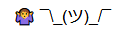
\includegraphics[height=4mm]{emoji-shrug}, indicating they are equally unsure about all possibilities.

The choice of priors is a choice the Bayesian modeler must make. There is no fundamental truth. But luckily there is some help, for example the Stan Devs have a great tutorial providing recommendations on choice of priors \cite{StanwikiPriors2019}:
\begin{itemize}
\item Flat prior;
\item Super-vague but proper prior: normal(0, 1e6);
\item Weakly informative prior, very weak: normal(0, 10);
\item Generic weakly informative prior: normal(0, 1);
\item Specific informative prior: normal(0.4, 0.2) or whatever. Sometimes this can be expressed as a scaling followed by a generic prior: \\$\theta = 0.4 + 0.2*z$, $z\sim$ normal(0, 1).
\end{itemize}


\begin{marginfigure}
    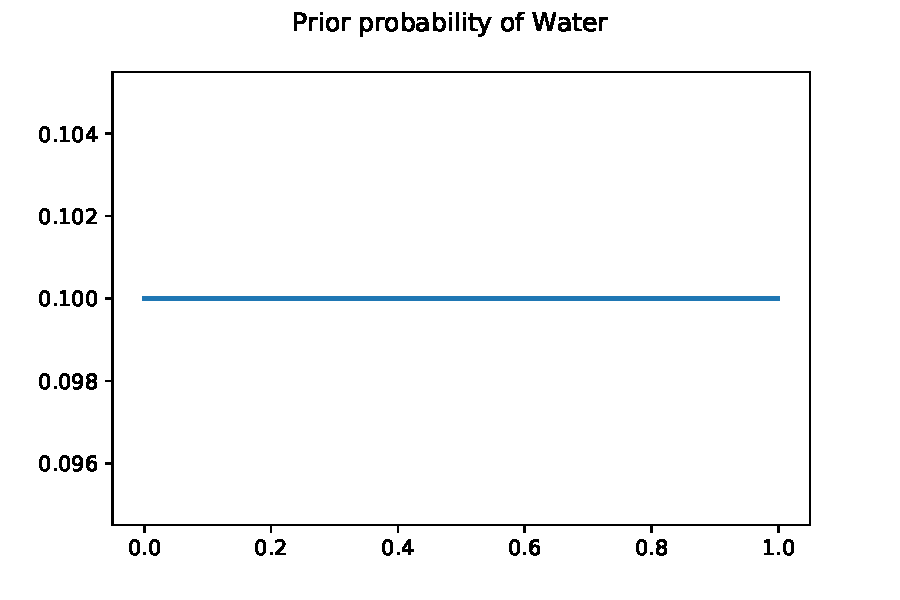
\includegraphics{bayesglos01}
    \caption{Prior probability of \lstinline{Water} is 0.1}
    \end{marginfigure}


\begin{lstlisting}
    # Create a prior in numpy
    possible_proportion_of_water = np.linspace(0,1,100)
    probability_of_possible = np.repeat(.1, 100)
    
    fig,ax=plt.subplots()
    ax.plot(possible_proportion_of_water, probability_of_possible)
    fig.suptitle("Prior probability of Water")
    plt.savefig('bayesglos01.pdf')
\end{lstlisting}

\newthought{The likelihood} is the probability of data, given a model and parameters.  
Assuming a binomial model, the likelihood of $W$ water events out of $N$ tosses, with proportion of \lstinline{Water} of $p$ is given by
\begin{equation}
P(W|N,p) = \frac{N!}{W!(N-W!)}p^W(1-p)^{N-W}
\end{equation}
The likelihood of $W$=6 \lstinline{Water} events given $N$=9 tosses, with a proportion of water of $p$=0.5 can be calculated
\begin{lstlisting}
count_of_water_observation = 6
count_of_tosses = 9
likelihood = stats.binom.pmf(k=count_of_water_observation,
                             n=count_of_tosses, p=.5)
print(f'likelihood={likelihood}')    
>>> likelihood=0.16406250000000006
\end{lstlisting}
The likelihood of $W$=6 \lstinline{Water} events given $N$=9 tosses, for all possible values of $p$ (between 0 and 1) can be calculated as shown in the graph.
\begin{marginfigure}
    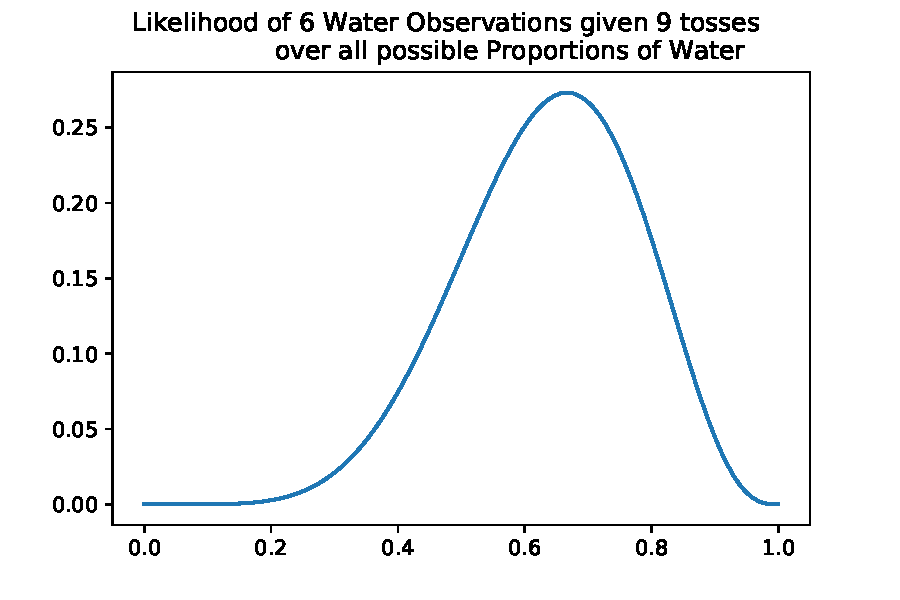
\includegraphics{bayesglos02}
    \caption{Likelihood of 6 out of 9 tosses being water for $0\leq p\leq 1$}
    \end{marginfigure}
\begin{lstlisting}
likelihood = stats.binom.pmf(k=count_of_water_observation, 
n=count_of_tosses,
p=possible_proportion_of_water)
fig,ax=plt.subplots()
ax.plot(possible_proportion_of_water, likelihood)
fig.suptitle("Likelihood of 6 Water Observations given 9 tosses \n \
over all possible Proportions of Water")
plt.savefig('bayesglos02.pdf')
\end{lstlisting}

\textbf{Note:} Likelihood is not a probability distribution, meaning that the total area of the curve is not equal to 1. This is why the syntax 
${\cal L}(\textrm{data}|\textrm{parameters})$
can be a bit more clear than $P(\textrm{data}|\textrm{parameters})$


\newthought{Marginal Likelihood of Evidence/Evidence/Average Likelihood}.
The ''Bayesian way'' to compare competing models $\alpha_i$ is to compute the marginal likelihood of each model $p(\textrm{data}|\alpha_1)$, i.e. the probability of the observed data $\textrm{data}$ given the $\alpha_i$ model \cite{PyMC3marglikeli2019}.

The marginal likelihood, also known as the evidence, or model evidence, is the denominator of the Bayes equation. Its only role is to guarantee that the posterior is a valid probability by making its area sum to 1. It is a likelihood function in which some parameter variables have been marginalized (integrated or summed out). 
If $\theta$ is the parameter being marginalised 
\begin{equation}
P(\textrm{data}|\alpha) = \int_\theta p(\textrm{data}|\theta)P(\theta|\alpha)d\theta
\end{equation}
Integrate the data given a parameter, weighted by the parameter value.

We can see the normalising effect if we write Bayes' theorem and make explicit the fact that all inferences are model-dependant.
\begin{equation*}
    P(\textrm{parameters}|\textrm{data},\alpha_i) = 
    \frac{P(\textrm{data}|\textrm{parameters},\alpha_i)P(\textrm{parameters}|\alpha_i} {P(\textrm{data}|\alpha_i)}
\end{equation*}

In most inference methods however this term is readily ignored, and ends up being derived out of the inference. The reason being its non trivial to calculate analytically, and very hard to simulate in multi-dimensional problems.


From \cite{Quoramarginallikelihoodandposterior2019}:
The marginal likelihood's only role is to guarantee that the posterior is a valid probability by making its area sum to 1.
Therefore, its only effect in the posterior is that it scales it up or down, but the shape of the posterior does not change.
Here you have the Bayes formula to get a posterior distribution. I express it in different ways in case some of the expressions is more familiar to you:
\begin{eqnarray}
\overbrace{p(\boldsymbol{\theta} | \mathbf{X})}^{\text { posterior }}
&=&
\frac{\overbrace{p(\mathbf{X} | \boldsymbol{\theta}) p(\boldsymbol{\theta} | \alpha)}^{\text { likelihood prior }}}
{
    \underbrace{ \int_{\boldsymbol{\theta}} p(\mathbf{X} | \boldsymbol{\theta}) p(\boldsymbol{\theta} | \alpha)}_{\text { marginal likelihood }}
    }\nonumber\\
&=& \frac{
    \overbrace{p(\mathbf{X} | \boldsymbol{\theta})}^{\text { likelihood}}
    \overbrace{p(\boldsymbol{\theta} | \alpha)}^{\text {prior }}
    }{
        \underbrace{p(\mathbf{X} | \alpha)}_{\text { marginal likelihood }}
        }\nonumber\\
&=&\frac{\overbrace{p(\mathbf{X}, \boldsymbol{\theta})}^{\text { joint probability }}}
{
    \underbrace{p(\mathbf{X} | \alpha)}_{\textrm{marginal likelihood}}
    }
\nonumber\\
&=&K p(\mathbf{X}, \boldsymbol{\theta}) \nonumber\\
&\propto& p(\mathbf{X}, \boldsymbol{\theta})\nonumber
\end{eqnarray}
where the $\alpha$ parameter that controls the prior is often implicit and we just write things like $p(\boldsymbol{\theta})$  or $p(\mathbf{X})$. As you can see, the marginal likelihood (marginal means that we marginalised, integrated, the variable $\boldsymbol{\theta}$) is different from the posterior. It is only one of the three elements needed to get the exact posterior.



Therefore the  Bayes formula often written where the denominator is removed, and a proportional to is shown rather than an equal:
\begin{equation*}
    P(\textrm{parameters}|\textrm{data},\alpha_i) \propto
    P(\textrm{data}|\textrm{parameters},\alpha_i)P(\textrm{parameters}|\alpha_i)
\end{equation*}
For our globe tossing example we are able to calculate the Marginal Likelihood because we are using a Grid Search Inference method can use the formulation below.
\begin{lstlisting}
    # Marginal Likelihood in Grid Search formulation
    numerator  = possible_proportion_of_water * likelihood
    denominator = sum(numerator)
    denominator
    
    6.300000720691165
    
\end{lstlisting}

\newthought{The posterior, or posterior probability}, is the probability of model parameters after incorporating the data. In the our water example, prior to the experiment, we were equally sure, (or unsure) what the proportion of water on the planet was. After using our model in conjunction with the data, we the posterior distribution reflects our certainty in the parameters.

Note that the posterior distribution is a distribution of possible model parameters and not a distribution of data.

This example is very nicely explained in McElreath's book \cite[Chapter 2]{McElreath2015} and video series.

\begin{lstlisting}
posterior = numerator/denominator
fig, axes =plt.subplots(1,2, figsize=(12,5))
axes[1].plot(possible_proportion_of_water, posterior)
axes[1].set_title("Posterior Probability of Proportion of Water")
axes[0].plot(possible_proportion_of_water, probability_of_possible) 
axes[0].set_title("Prior Probability of Proportion of Water")
plt.savefig('bayesglos03.pdf')
\end{lstlisting}
\begin{figure*}[h]
    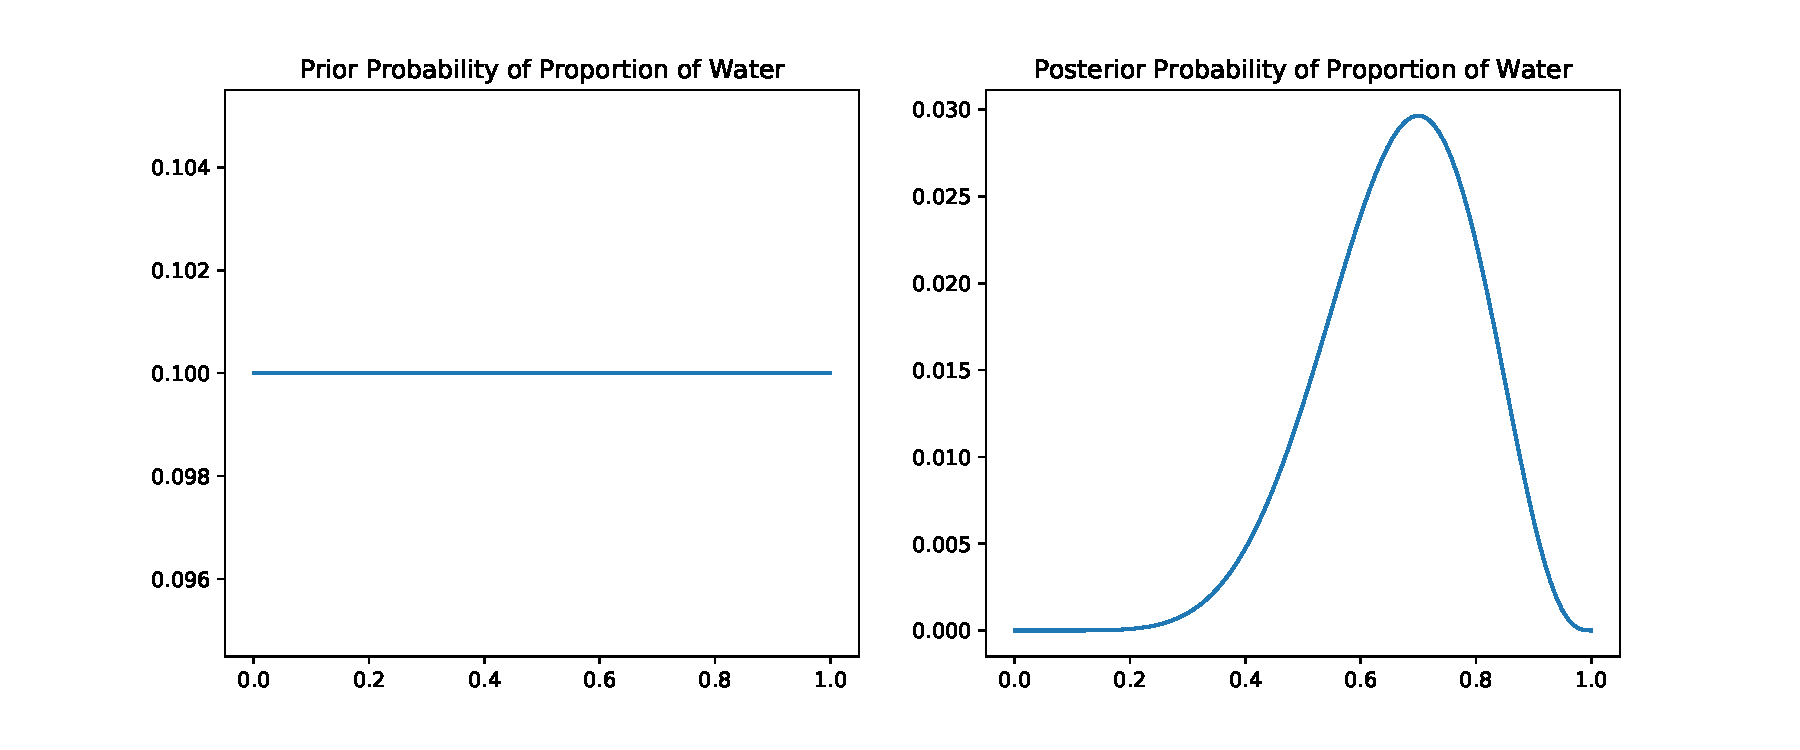
\includegraphics[width=0.56\textwidth]{bayesglos03}
    \caption{Prior and posterior probability of water}
    \end{figure*}

\newthought{Posterior Predictive} 
An advantage of Bayesian models is being able to calculate data after the model has been updated. The simulation of data, taking into account observed data, is called the posterior predictive. The mathematical formulation is as follows.
\begin{equation}
    \operatorname{Pr}\left(y^{\prime} | y\right)=\int \operatorname{Pr}\left(y^{\prime} | \theta\right) \operatorname{Pr}(\theta | y) d \theta
    \end{equation}
We can simulate the posterior predictive distribution using python. 
\begin{lstlisting}
posterior_samples = np.random.choice(possible_proportion_of_water, p=posterior, size=1000, replace=True)
posterior_predictive = stats.binom.rvs(n=9, p=posterior_samples)
counts = np.bincount(posterior_predictive)

fig, ax = plt.subplots()
ax.bar(x=np.arange(counts.shape[0]), height=np.bincount(posterior_predictive))
ax.set_xlabel("Count of Water Observations out of 9 globe tosses")
ax.set_ylabel("Number of simulations with count")
plt.savefig('bayesglos04.pdf')
\end{lstlisting}

\begin{marginfigure}
    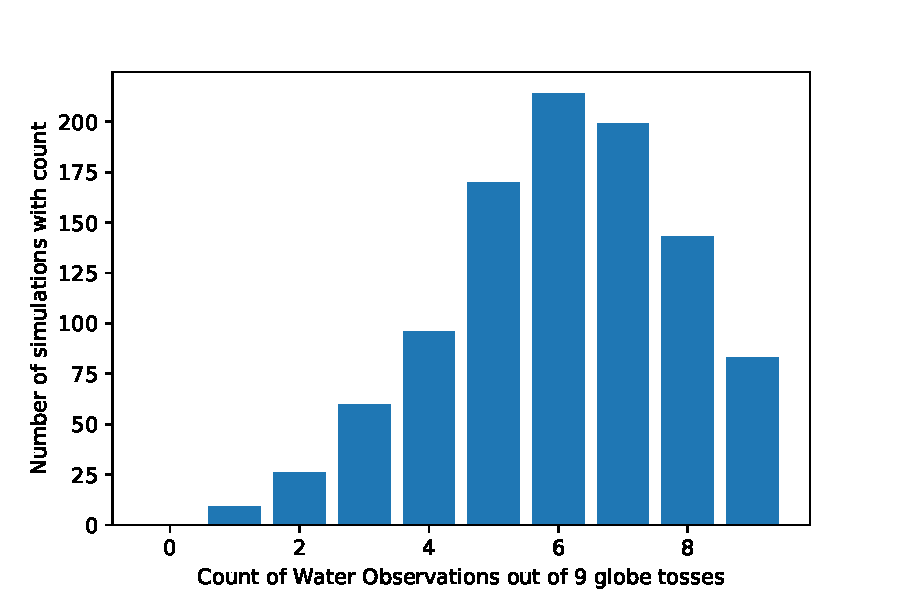
\includegraphics{bayesglos04}
    \caption{Posterior Predictive}
    \end{marginfigure}

It is important to note that this distribution is not probability. It is in the units of data, in this case it is the distribution of ''counts of water observations for 9 globe tosses''. The distribution highlights the uncertainty in the globe outcome given the 9 data points that were originally observed.

\newthought{Prior Predictive Distribution}. 
Prior Predictive models are similar to posterior predictive distributions, except that you use samples from the prior distribution of parameters, not from the posterior distribution of samples.
\begin{equation}
    p(y)=\int_{\theta} p(\theta) p(y | \theta) \mathrm{d} \theta
    \end{equation}
Prior Predictive distributions are useful for checking if your model seems to be outputting reasonable data, for example in our globe tossing experiment, if we were seeing negative counts for ''Number of water observations'', that impossibility would suggest that the model is not appropriate for the data
\begin{lstlisting}
    prior_samples = stats.uniform(0,1).rvs(1000)
    prior_predictive_samples = stats.binom.rvs(n=9, p=prior_samples)
    counts = np.bincount(prior_predictive_samples)
    
    fig, ax = plt.subplots()
    ax.bar(x=np.arange(counts.shape[0]), height=np.bincount(prior_predictive_samples))
    ax.set_xlabel("Count of Water Observations out of 9 globe tosses")
    ax.set_ylabel("Number of simulations with count")
    plt.savefig('bayesglos05.pdf')
\end{lstlisting}

\begin{marginfigure}
    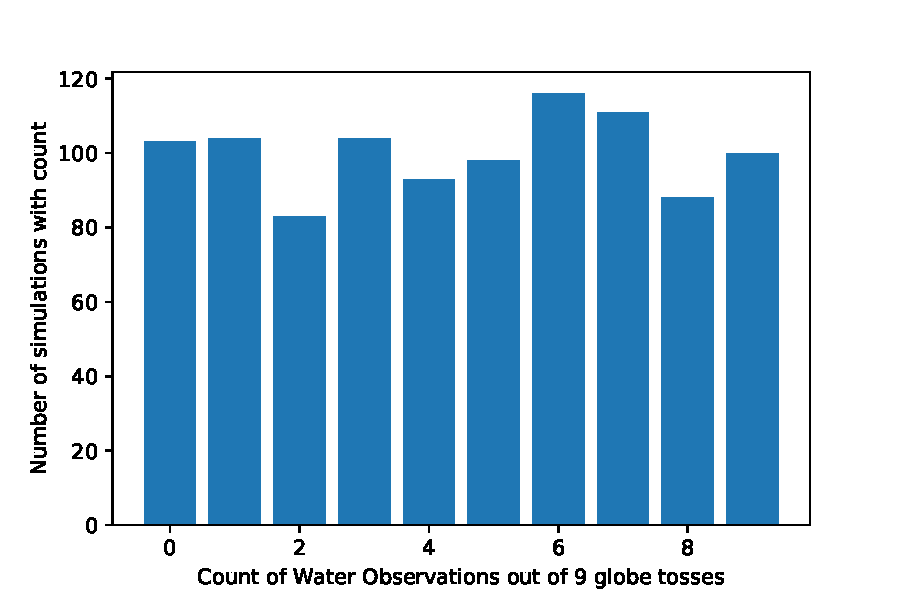
\includegraphics{bayesglos05}
    \caption{Posterior Predictive}
    \end{marginfigure}

\newthought{Forward Sampling} is the same as Prior Predictive except that it includes the prior samples. Whereas Prior Predictive is just the distribution of simulated data, Forward Sampling is that in addition to the sampled parameters from the posterior.

\newthought{Hierarchical modelling} is a mechanism in Bayesian models where you ''tell'' the model that data points may share similarity. The hierarchy words implies multiple ''levels'' of effect.

For example assume you're trying to estimate the height of an individual. Your data tells you the gender and which family the individual comes from. The relation between height and family is not constant, it's not as if coming from one family guarantees all members of a family will be double the height of another for example. But it would be unwise to assume that your samples are independent either, family genetics is well correlated with final height. But with hierarchical models allow us to split the difference, by allowing the model to ''say'' a families heights come from a taller distribution, than from another family with shorter family members.

The Radon Model \cite{PyMC3multilevel2019} provides a rigorous explanation accompanied by a great visual explainer

\newthought{Hierarchical Funnel}

% Hierarchical funnels are a particular parameter space topology that makes it hard for particular Inference Engines to explore the whole space. Basically what ends up happening is this, where the Bayesian sampler doesn't quite do the thing you want, but instead of your donation coin taking a long time to fall a short vertical distance, your sampler can't traverse the entire space efficiently.

Michael Betancourt wrote a full explanation on the Stan website \cite{MichaelBetancourtdivergence2017}. The tutorial has also been rewritten in PyMC3 \cite{PyMC3Divergences2019}.


\section{Acknowledgements}

I would like to extend thanks to the following people for providing feedback and corrections
\begin{lstlisting}
George Ho (Twitter: @_eigenfoo)
Alexander Etz (Twitter: @AlxEtz)
Ari Hartikainen (Twitter: @a_hartikainen)
\end{lstlisting}

